\documentclass[20pt,margin=1in,innermargin=-4.5in,blockverticalspace=-0.25in]{tikzposter}
\geometry{paperwidth=42in,paperheight=32.5in}
\usepackage[utf8]{inputenc}
\usepackage{amsmath}
\usepackage{amsfonts}
\usepackage{amsthm}
\usepackage{amssymb}
\usepackage{mathrsfs}
\usepackage{graphicx}
\usepackage{adjustbox}
\usepackage{enumitem}
\usepackage[backend=biber,style=ieee,sorting=none]{biblatex}
\usepackage{uomtheme}

\usepackage{float}

\usepackage{mwe} % for placeholder images

\addbibresource{refs.bib}

% set theme parameters
\tikzposterlatexaffectionproofoff
\usetheme{UoMTheme}
\usecolorstyle{UoMStyle}

\usepackage[scaled]{helvet}
\renewcommand\familydefault{\sfdefault} 
\usepackage[T1]{fontenc}


\title{Developing a Haskell Optics Manipulation Tool}
\author{Mateo Borina}
\institute{Juraj Dobrila University of Pula, Faculty of informatics}
\titlegraphic{
\includegraphics[width=0.12\textwidth]{unipufipulogos.png}}

% begin document
\begin{document}
\maketitle
\centering
\begin{columns}
    \column{0.32}
    \block{Optics in Haskell}{
        \textbf{Optics} in Haskell simplify data manipulation through a unified and composable interface for working with complex structures \cite{riley2018categories}. Optics include different types:\\
        
        \begin{itemize}
            \item \textbf{Lens:} Focuses on getting and setting values.
            \item \textbf{Prism:} Handles optional values.
            \item \textbf{Traversal:} Generalizes mapping over multiple elements.
            \item \textbf{Iso:} Represents bidirectional type conversion.
        \end{itemize}
        
        \hfill \break \textbf{Features:}
        \begin{itemize}
            \item Composability: Combining optics for complex data manipulation.
            \item Readability: Enhancing code clarity and maintainability.
        \end{itemize}
        
        \textbf{Benefits:}
        \begin{itemize}
            \item Type System Integration: Ensuring correctness and maintainability.
            \item Functional Style: Encouraging a modular, functional programming approach.
        \end{itemize}
        
        \begin{center}
        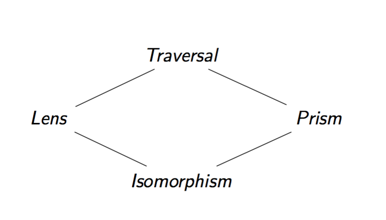
\includegraphics[width=0.12\textwidth]{composition.png}
        \end{center}
    }
    
    \block{Problem}{
        In functional programming, particularly within the Haskell ecosystem, data manipulation can become \textbf{complicated} when dealing with complex structures \cite{roman2020profunctor}. Traditional approaches may lead to \textbf{less maintainable code}. This project addresses the challenge of \textbf{enhancing the clarity and modularity} of data manipulation in Haskell by developing a specialized optics manipulation tool, simplifying the process and promoting a \textbf{more expressive coding style}.
        \hfill \break
    }
    
    \block{Objectives}{
        \textbf{Tool Development}

        Create a Haskell optics manipulation tool for simplified handling of complex data structures.
        \hfill \break
        
        \textbf{Enhanced Modularity}
        
        Improve code modularity with a user-friendly interface for concise, maintainable Haskell programs.
        \hfill \break
        
        \textbf{Improved Readability}
        
        Enhance code readability by simplifying complex data manipulations using the developed tool.
        \hfill \break
        
        \textbf{Efficient Data Navigation}
        
        Enable precise navigation and manipulation of complex data structures through optics implementation.
        \hfill \break
        
        \textbf{Community Contribution}
        
        Contribute to functional programming by providing a specialized solution for Haskell optics-based transformations.
        \hfill \break
    }

    \column{0.36}
    
    \block{Methodology}{
        \textbf{Problem-Focused Optics Manipulation Module (OpticsManipulation.hs)}
        \begin{itemize}
            \item Tackles data manipulation challenges through lenses, prisms, traversals, and isomorphisms for efficient operations on diverse data structures.
            \item Defines specific optics for structured data types, simplifying navigation and modification of complex information.
            \item Implements functions for composing and chaining optics, enabling modular transformations to meet precise data manipulation needs.
            \item Ensures robustness with error-handling mechanisms within optics, protecting against unexpected input scenarios.
            \item Includes concise helper functions for common tasks, enhancing code clarity in traversing, modifying, and rounding values.
            \item Defines isomorphisms and functions for bidirectional type conversions, easing tasks like temperature unit conversion.
        \end{itemize}
        
        \begin{center}
        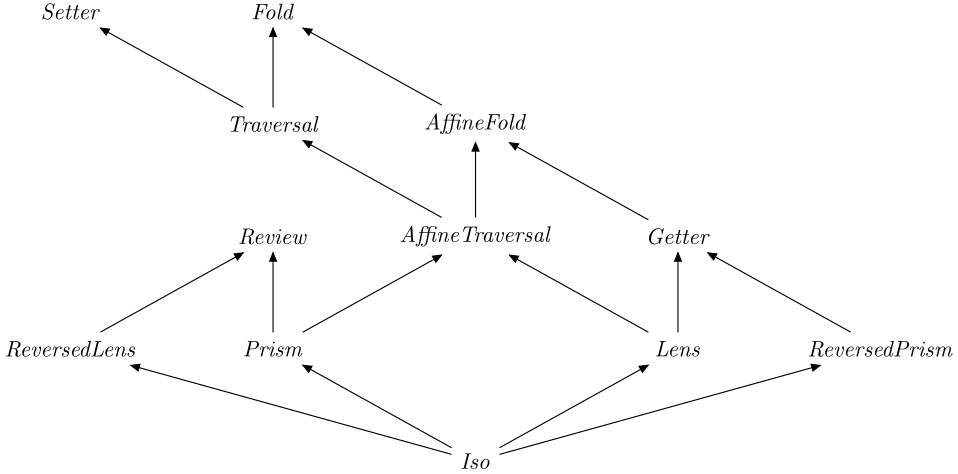
\includegraphics[width=0.35\textwidth]{optics.png}
        \end{center}
    }
    
    \block{Implementation}{
        Characteristics of the \textbf{module implementation}:

        \begin{itemize}
            \item The module, named \textbf{OpticsManipulation}, encapsulates various optics types and functions, including lenses, prisms, traversals, and isomorphisms.
            \item Defines \textbf{sample data types} to demonstrate the application of optics for structured data manipulation.
            \item Presents lens, prism, and traversal types with associated \textbf{creation functions}.
            \item Provides functions for \textbf{composing and chaining} optics to create more complex transformations.
            \item Implements \textbf{functions for modifying values} through optics with error handling, emphasizing a robust approach to data manipulation.
            \item Includes \textbf{helper functions} for traversing, modifying, and rounding values within a structure.
            \item Introduces \textbf{isomorphism types and associated functions} for bidirectional type conversions.
            \item Demonstrates the creation of \textbf{sample isomorphisms} for temperature conversion.
        \end{itemize}
    }

    \column{0.32}
    
    \block{Results and documentation}{
        \textbf{Main Function and examples (MainFunction.hs)}
        \begin{itemize}
            \item Illustrates practical application through a main function with examples, showcasing the tool's efficiency in solving the problem.
            \item Prioritizes error handling is prioritized in optics-based modifications, ensuring reliability and resilience to errors in unexpected scenarios.
        \end{itemize}
        
        \textbf{Documentation}\\
        Provides clear, concise and detailed documentation for functions, data types, and examples, enhancing accessibility and ease of maintenance.
        \hfill \break
    }
    
    \block{Discussion}{
        \textbf{Learning solution}\\
        Developing the Haskell Optics Manipulation Tool serves as a valuable learning solution for navigating and modifying data in functional programming. While acknowledging the existence of similar tools \cite{Gundry_Loh_Rybczak_Grenrus}, this project emphasizes clarity and educational value.
        \hfill \break
        
        \textbf{Challenges and limitations}\\
        Challenges in error handling and optimization present opportunities for further refinement. Additionally, there are ways of expanding the tool such as adding support for more optics types, enhancing composition and optimizing the algorithms.
        \hfill \break
    }
    
    \block{Conclusion}{
        In conclusion, Haskell Optics Manipulation Tool empowers Haskell developers with a versatile toolkit for effective data manipulation. The modular design of lenses, prisms, and traversals facilitates precise and concise transformations. This project not only provides practical solutions to real-world challenges but also stands as an educational resource, contributing to the growth and understanding of optics in the Haskell programming language.
        \hfill \break
    }
    
    \block{Materials}{
        Haskell: \url{https://www.haskell.org/}
        \hfill \break
        LaTeX: \url{https://www.latex-project.org/}
        \hfill \break
        Codebase, documentation, and this poster: \url{https://github.com/b0rke-mborina/optics-manipulation-tool}
        
        \begin{center}
        
\includegraphics[width=0.072\textwidth]{frame.png}
        \end{center}
    }
    
    \block{References}{
        \vspace{-1em}
        \begin{footnotesize}
        \printbibliography[heading=none]
        \end{footnotesize}
    }
\end{columns}
\end{document}